\section{Introduction}
\label{sec:introduction}

%\MW{We need still an appealing and convincing introduction. I think this is the best part for you to write. While doing this, you might want to look at the following section and remove all the repetitions in there.}


Ageing has started to impact the labour markets profoundly, and robotic labour shortage relief is becoming a necessity in all industries~\cite{mcgrath2021report,astrov2021economies}. Yet, there are still surprisingly few robots operating outside of structured environments. To bring robots successfully to human-occupied environments, the main challenge still is handling human-instilled disturbances~\cite{rodriguez2021human}, e.g., misplaced products in shelves, newly added products, blocked aisles, or interactions from humans. Such disturbances should be handled adaptively, with little development effort and short response times for natural effective interaction. 
Focusing on these challenges, this paper demonstrates a combination of two novel methods, one for adaptive decision making and one for rapid motion planning, embedded in a state-of-the-art integrated robot system. 

The demonstrator is a mobile manipulator for order picking in realistic supermarkets, see \cref{fig:layouts}. %In the following, we explain how this demonstrator is rooted in a real need. 
The increase in online shopping  induces an equal decrease in store visits. Especially in dense urban areas, these costly but conveniently located stores could have a dual use as distribution centres for flash delivery of online orders \cite{kronmuller2023online}. This requires the order picking to occur during opening hours, amongst store customers. We have taken this as our demonstrator scenario, but the methods are generally applicable for any scenario involving human-disturbed mobile manipulation tasks. In such scenarios, we assume that humans can block the robot's path, physically push or hold the manipulator, and move the pick-able items, before, during, or after a pick. Even if items are taken away from the robot's suction gripper, it should recover by picking another item of the same product. % of the same kind.
%

\begin{figure}
  \centering
  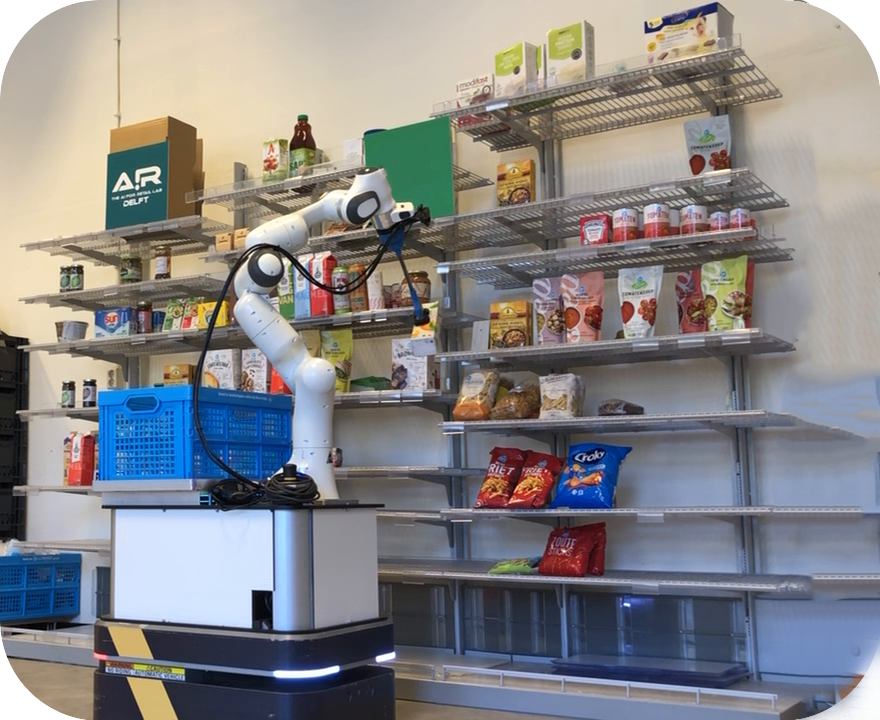
\includegraphics[height=140pt]{layout_lab_wo.png}
  \caption{We validated our mobile manipulator in our AIRLab lab environment (shown here) and a realistic supermarket environment of a large Dutch retailer. %Robot Hardware used for in the demo in the two evaluated environments. 
  %The robot is
  %composed out of a differential-drive robotic base and a
  %7-dof robotic arm.}
  }
  \label{fig:layouts}
\end{figure}
%Past demo papers at RSS, \cite{li2023large,deepmind2023demonstrating,toyota2023}

%Although the realization of such an %application is deemed simple
% To deploy autonomous robots in supermarkets with success, their operation in a
% human-shared environment must be safe, 
% fault-tolerant, and adaptive.
In this work, we present our solution to mobile manipulation
in human-shared environments that aims at being adaptive and fault-tolerant. %Doing so, 
We  focus on three main questions that we argue are most 
relevant when deploying robots in supermarkets:

\begin{enumerate}
  \item How can we generate \emph{safe} and \emph{robust} trajectories for manipulation? % (safety, robustness)? %be robust, safe and easy to adapt by
  %non-experts (ease-of-use)?
  \item How can we ensure \emph{fault-tolerant} task planning and execution? % (fault-tolerance)? 
  \item How can we easily \emph{adapt} the robot to pick new products? % (adaptability)?
  %data-driven item detection be extended quickly (extendability)?
\end{enumerate}
Our solution addresses these questions with specific decisions on the robot's capabilities for decision-making, trajectory generation, and perception. Our contributions are thus an integrated system with adaptive decision-making, fast motion planning and easy-to-use teaching from demonstration. 

%Each of these points is mainly effected by one component, decision making, trajectory generation and perception respectively. 
% Thus, the motivational questions were the driver to our design decisions.

% \subsection{Assumptions in the context of supermarkets}

% Modern retails and supermarkets have access to a detailed information of all
% products, this includes mass, geometry and location in the store. In this paper,
% we assume that the robot can access this database to inform its decision.
% Supermarkets are characterized by a large range of products, around 100.000
% different products per store.  This work deliberately excludes
%  products that require specialized grasping strategies or even specific hardware design in favor of reliability for the remaining products.
% Moreover, in the interest of bridging the gap between robotics research and
% applications on the market, achieving high reliability for a part of all
% products is assumed to be favorable. Besides, we assume that products to
% pick are visible from the front of the shelf. We explicitly focus on
% in-store-picking during opening-hours, because warehouse automation is already
% being tackled by redesigning the interior making collaborative robots obsolete
% in such environments. Based on this focus, we generally favor reliability over
% execution speed. 

%To address these question we go through the different modules of our system \ref{sec:order_system_overview}. Chapter \ref{sec:decision_making} introduces our adaptive decision making solution. Chapter \ref{sec:trajectory_generation} covers we 
